\documentclass{standalone}
\usepackage{tikz}
\usepackage{standalone}
\begin{document}
	
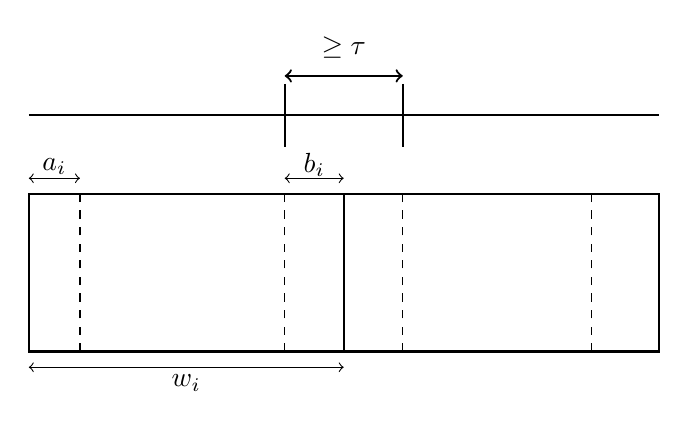
\begin{tikzpicture}
%\draw [help lines] (-1,-2) grid (9,5);

\draw [thick] (0,3) -- (8,3);
\draw [thick] (3.25,3.4) -- (3.25,2.6);
\draw [thick] (4.75,3.4) -- (4.75,2.6);
\draw [thick, <->] (3.25, 3.5) -- (4.75, 3.5);
\node [above] at (4,3.6) {$\geq \tau$};


\draw [thick] (0,0) rectangle (8,2);
\draw [thick] (4,2) -- (4,0);
\draw [dashed] (0.65,0) -- (0.65,2);
\draw [dashed] (3.25,0) -- (3.25,2);
\draw [dashed] (4.75,0) -- (4.75,2);
\draw [dashed] (7.15,0) -- (7.15,2);

%\draw [<->] (3.5,2.2) -- (4.5,2.2);
%\node at (4, -.4) {\scriptsize $\geq \tau$};

\draw [<->] (0,-.2) -- (4,-.2);
\node at (2, -.4) {$w_i$};


\draw [<->] (0, 2.2) -- (0.65, 2.2);
\node at (0.325, 2.35) {$a_i$};

\draw [<->] (3.25, 2.2) -- (4, 2.2);
\node at (3.625, 2.375) {$b_i$};





\end{tikzpicture}
	
\end{document}